\documentclass[./../main.tex]{subfiles}
\graphicspath{{img/}}

\begin{document}
    \section{}
    Dado el campo vectorial \(\vect{A} = xy\uveci + yz\uvecj + zx\uveck\), evaluar el flujo de \(\vect{A}\) a través de la superficie de un paralelepípedo rectangular de lados \(a\), \(b\), \(c\), con el origen de uno de los vértices y las aristas a lo largo de las direcciones positivas de los ejes rectangulares, tal como se muestra en la \cref{fig:surfaceProblem2}. Evaluar \(\displaystyle\int \dvg{\vect{A}}\odif{V}\) sobre el volumen de este mismo paralelepípedo y comparar resultados.

    \begin{figure}[htb]
        \centering
        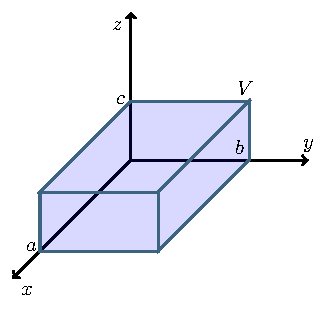
\includegraphics[scale=1.1]{diagram-problem-2.pdf}
        \caption{Diagrama correspondiente al problema 2.}
        \label{fig:surfaceProblem2}
    \end{figure}
\end{document}